\section{Tập dữ liệu thứ nhất}

\subsection{Giới thiệu về tập dữ liệu}

\subsubsection{Breast Cancer Wisconsin (Diagnostic)}
Đây là một tập dữ liệu nổi tiếng trong lĩnh vực học máy và phân tích dữ liệu y tế, được thiết kế để phân loại khối u vú là \textbf{lành tính (Benign)} hoặc \textbf{ác tính (Malignant)} dựa trên các đặc trưng số học được trích xuất từ hình ảnh tế bào.


\subsubsection{Thông tin tổng quan về tập dữ liệu}

\begin{itemize}
	\item \textbf{Nguồn gốc}: UCI Machine Learning Repository.
	\item \textbf{Mục đích}: Phân loại khối u vú là \textit{lành tính} (benign) hoặc \textit{ác tính} (malignant).
	\item \textbf{Số mẫu}: 569.
	\item \textbf{Số đặc trưng}: 30 đặc trưng đầu vào (dạng số học):
	\begin{enumerate}
		\item \textbf{Bán kính (radius)}.
		\item \textbf{Kết cấu (texture)}.
		\item \textbf{Chu vi (perimeter)}.
		\item \textbf{Diện tích (area)}.
		\item \textbf{Độ nhẵn (smoothness)}.
		\item \textbf{Độ gọn (compactness)}.
		\item \textbf{Độ lồi (concavity)}.
		\item \textbf{Số điểm lõm (concave points)}.
		\item \textbf{Đối xứng (symmetry)}.
		\item \textbf{Kích thước phân dạng (fractal dimension)}.
	\end{enumerate}
	
	\item \textbf{Nhãn đầu ra}:
	\begin{itemize}
		\item \textbf{0}: \textit{Lành tính (Benign)}.
		\item \textbf{1}: \textit{Ác tính (Malignant)}.
	\end{itemize}
\end{itemize}


\subsubsection{Phân phối lớp}

Tập dữ liệu \textbf{Breast Cancer Wisconsin (Diagnostic)} có 569 mẫu, trong đó:

\begin{itemize}
	\item \textbf{Lành tính(Benign)}: 357 mẫu, chiếm 37.3\% trong 569 mẫu. 
	\item \textbf{Ác tính(Malignant)}: 212 mẫu. chiếm 62.7\% trong 569 mẫu.
\end{itemize}


\subsection{Tiền xử lý dữ liệu}

\subsubsection{Chia dữ liệu huấn luyện và dữ liệu kiểm tra}

\begin{itemize}
	\item 40\% tập huấn luyện, 60\% tập kiểm tra.
	\item 60\% tập huấn luyện, 40\% tập kiểm tra.
	\item 80\% tập huấn luyện, 20\% tập kiểm tra.
	\item 90\% tập huấn luyện, 10\% tập kiểm tra.
\end{itemize}

Quá trình chia dữ liệu được thực hiện bằng cách sử dụng hàm \textbf{train\_test\_split} từ thư viện \textbf{sklearn.model\_selection}. Hàm này đảm bảo rằng việc chia dữ liệu là ngẫu nhiên và đồng nhất. Ví dụ cách sử dụng:

\begin{verbatim}
	from sklearn.model_selection import train_test_split
	
	# Chia dữ liệu với tỷ lệ 80/20
	X_train, X_test, y_train, y_test = train_test_split(X, y, test_size=0.2, 
																																																											random_state=42)
\end{verbatim}

Trong đó:
\begin{itemize}
	\item \texttt{X}: Ma trận đặc trưng (features).
	\item \texttt{y}: Nhãn đầu ra (labels).
	\item \texttt{test\_size}: Tỷ lệ của tập kiểm tra so với dữ liệu tổng.
	\item \texttt{random\_state}: Giá trị cố định để đảm bảo kết quả chia dữ liệu có thể tái lập.
\end{itemize}

\textbf{Tỷ lệ 40/60}

\begin{itemize}
	\item \textbf{Tập huấn luyện}: 227 mẫu (142 Benign, 85 Malignant).
	\item \textbf{Tập kiểm tra}: 342 mẫu (215 Benign, 127 Malignant).
\end{itemize}

\begin{figure}[h!]
	\centering
	\begin{minipage}[b]{0.32\linewidth}
		\centering
		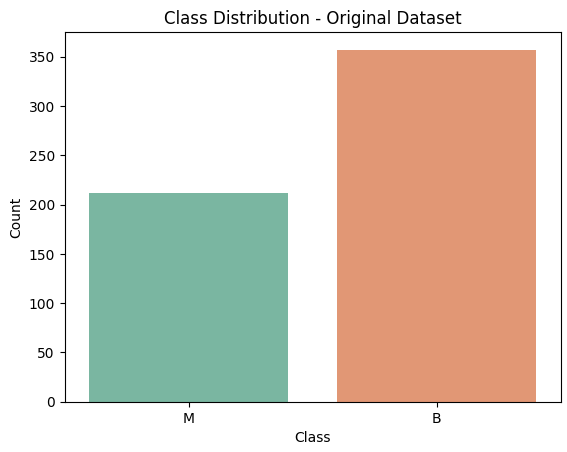
\includegraphics[width=\linewidth]{figures/dataset1/1.1.png}
		\caption{Original Dataset}
		\label{fig:original}
	\end{minipage}%
	\hfill
	\begin{minipage}[b]{0.32\linewidth}
		\centering
		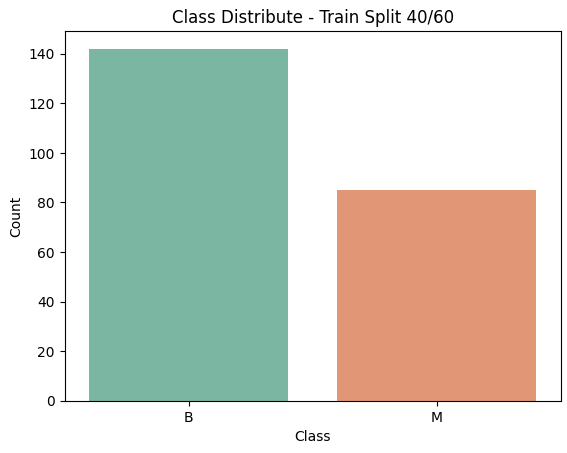
\includegraphics[width=\linewidth]{figures/dataset1/1.2.png}
		\caption{Training 40\%}
		\label{fig:train}
	\end{minipage}%
	\hfill
	\begin{minipage}[b]{0.32\linewidth}
		\centering
		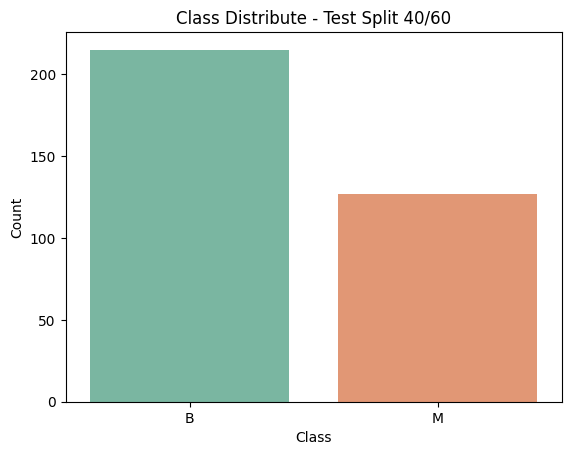
\includegraphics[width=\linewidth]{figures/dataset1/1.3.png}
		\caption{Test 60\%}
		\label{fig:test}
	\end{minipage}
	\caption{Phân phối lớp cho tỷ lệ chia 40/60.}
	\label{fig:split_40_60}
\end{figure}




\textbf{Tỷ lệ 60/40}

\begin{itemize}
	\item \textbf{Tập huấn luyện}: 341 mẫu (214 Benign, 127 Malignant).
	\item \textbf{Tập kiểm tra}: 228 mẫu (143 Benign, 85 Malignant).
\end{itemize}

\begin{figure}[h!]
	\centering
	\begin{minipage}[b]{0.32\linewidth}
		\centering
		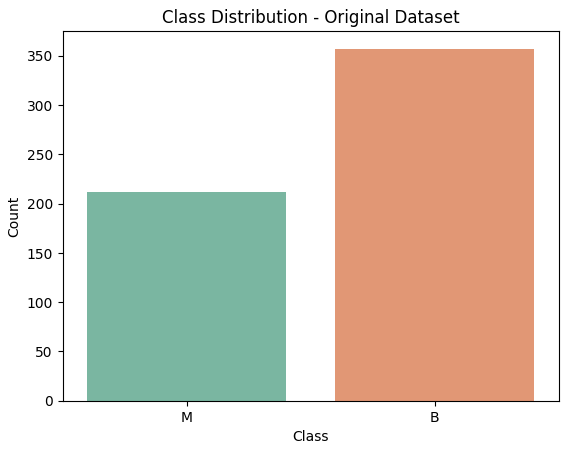
\includegraphics[width=\linewidth]{figures/dataset1/2.1.png}
		\caption{Original Dataset}
		\label{fig:original_1}
	\end{minipage}%
	\hfill
	\begin{minipage}[b]{0.32\linewidth}
		\centering
		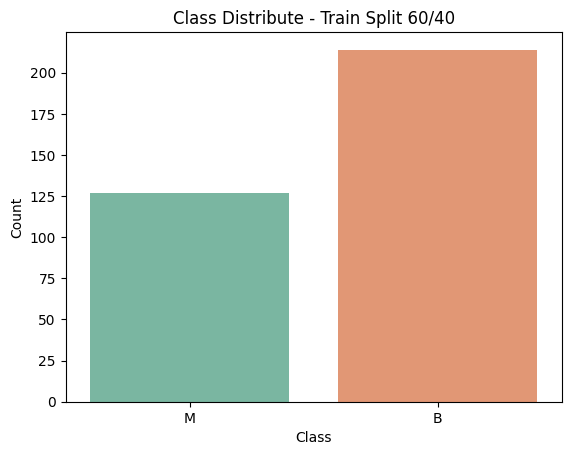
\includegraphics[width=\linewidth]{figures/dataset1/2.2.png}
		\caption{Training 60\%}
		\label{fig:train60}
	\end{minipage}%
	\hfill
	\begin{minipage}[b]{0.32\linewidth}
		\centering
		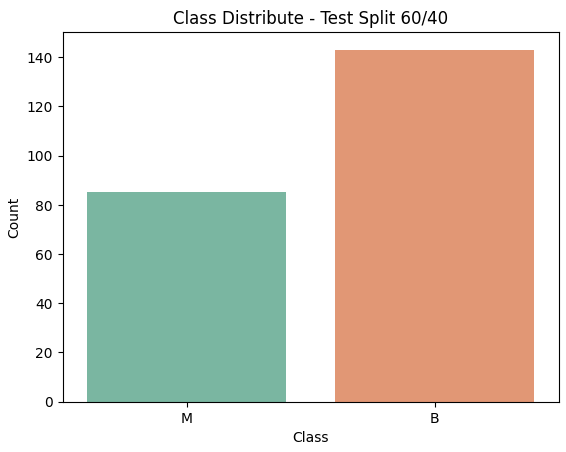
\includegraphics[width=\linewidth]{figures/dataset1/2.3.png}
		\caption{Test 40\%}
		\label{fig:test40}
	\end{minipage}
	\caption{Phân phối lớp cho tỷ lệ chia 60/40.}
	\label{fig:split_60_40}
\end{figure}

\newpage
\textbf{Tỷ lệ 80/20}

\begin{itemize}
	\item \textbf{Tập huấn luyện}: 455 mẫu (285 Benign, 170 Malignant).
	\item \textbf{Tập kiểm tra}: 114 mẫu (72 Benign, 42 Malignant).
\end{itemize}

\begin{figure}[h!]
	\centering
	\begin{minipage}[b]{0.32\linewidth}
		\centering
		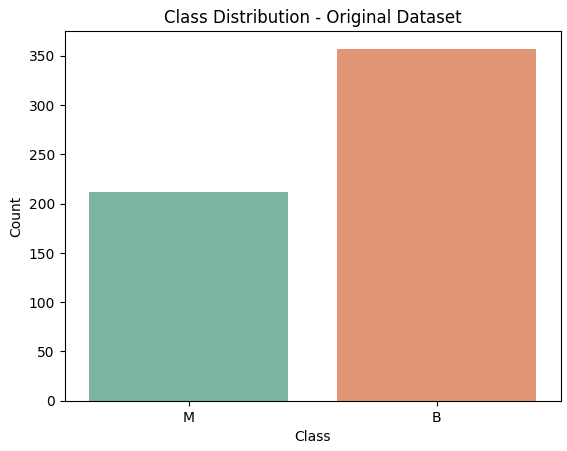
\includegraphics[width=\linewidth]{figures/dataset1/3.1.png}
		\caption{Original Dataset}
		\label{fig:original_2}
	\end{minipage}%
	\hfill
	\begin{minipage}[b]{0.32\linewidth}
		\centering
		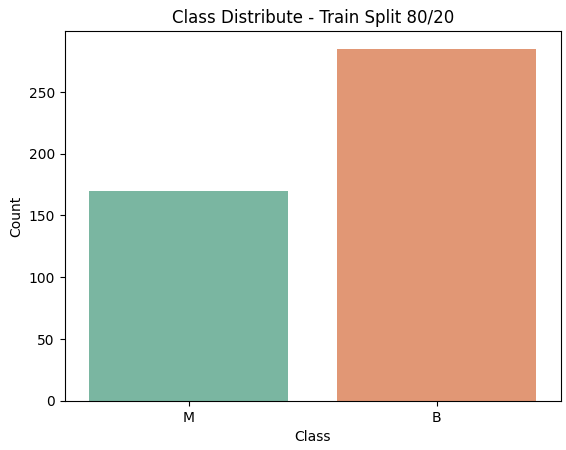
\includegraphics[width=\linewidth]{figures/dataset1/3.2.png}
		\caption{Training 80\%}
		\label{fig:train80}
	\end{minipage}%
	\hfill
	\begin{minipage}[b]{0.32\linewidth}
		\centering
		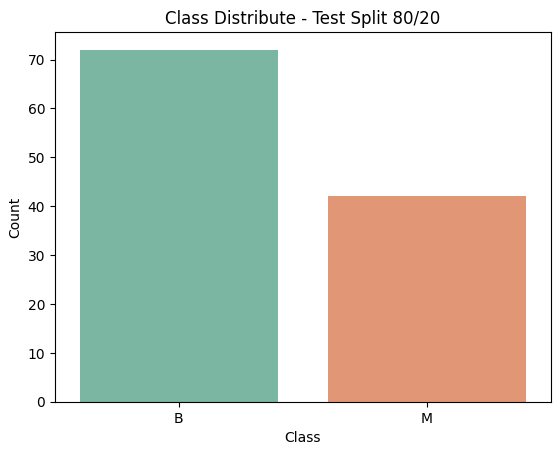
\includegraphics[width=\linewidth]{figures/dataset1/3.3.png}
		\caption{Test 20\%}
		\label{fig:test20}
	\end{minipage}
	\caption{Phân phối lớp cho tỷ lệ chia 80/20.}
	\label{fig:split_80_20}
\end{figure}


\textbf{Tỷ lệ 90/10}

\begin{itemize}
	\item \textbf{Tập huấn luyện}: 512 mẫu (321 Benign, 191 Malignant).
	\item \textbf{Tập kiểm tra}: 57 mẫu (36 Benign, 21 Malignant).
\end{itemize}

\begin{figure}[h!]
	\centering
	\begin{minipage}[b]{0.32\linewidth}
		\centering
		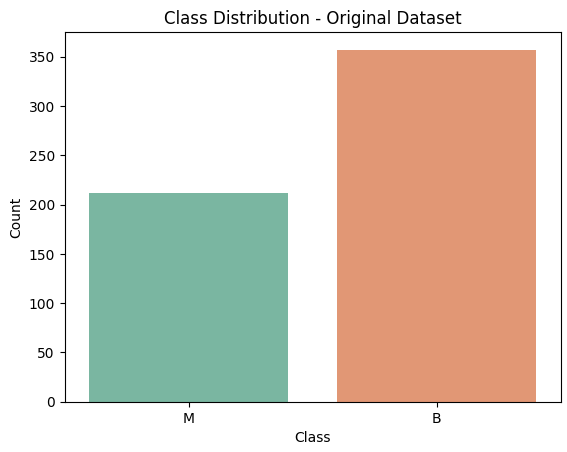
\includegraphics[width=\linewidth]{figures/dataset1/4.png}
		\caption{Original Dataset}
		\label{fig:original_3}
	\end{minipage}%
	\hfill
	\begin{minipage}[b]{0.32\linewidth}
		\centering
		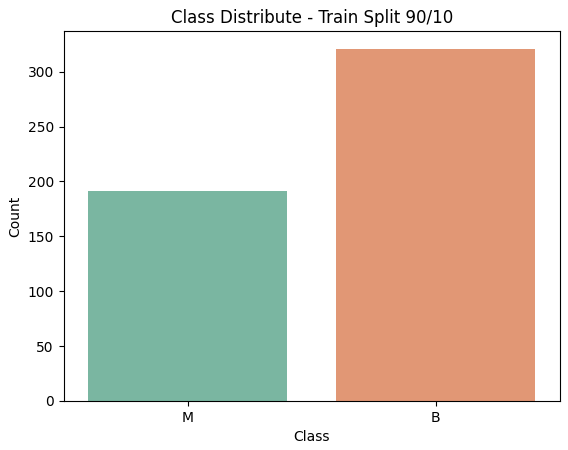
\includegraphics[width=\linewidth]{figures/dataset1/4.2.png}
		\caption{Training 90\%}
		\label{fig:train90}
	\end{minipage}%
	\hfill
	\begin{minipage}[b]{0.32\linewidth}
		\centering
		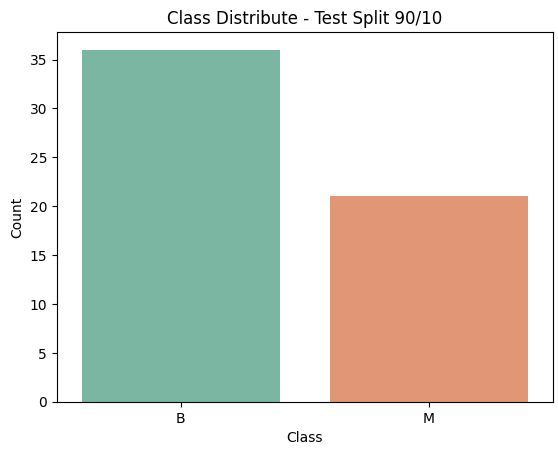
\includegraphics[width=\linewidth]{figures/dataset1/4.3.png}
		\caption{Test 10\%}
		\label{fig:test10}
	\end{minipage}
	\caption{Phân phối lớp cho tỷ lệ chia 90/10.}
	\label{fig:split_90_10}
\end{figure}
\newpage
\subsection{Phân tích các độ đo}

\subsubsection{Classification Report và Confusion Matrix (Train=40\%,Test=60\%)}

\textbf{Phân tích Classification Report}

\begin{table}[h!]
	\centering
	\begin{tabular}{|l|c|c|c|c|}
		\hline
		\textbf{} & \textbf{Precision} & \textbf{Recall} & \textbf{F1-Score} & \textbf{Support} \\ \hline
		\textbf{B} & 0.91 & 0.96 & 0.93 & 215 \\ \hline
		\textbf{M} & 0.92 & 0.83 & 0.88 & 127 \\ \hline
		\textbf{Accuracy} & \multicolumn{2}{c|}{} & 0.91 & 342 \\ \hline
		\textbf{Macro Avg} & 0.91 & 0.90 & 0.90 & 342 \\ \hline
		\textbf{Weighted Avg} & 0.91 & 0.91 & 0.91 & 342 \\ \hline
	\end{tabular}
	\caption{Classification Report với Train=40\% và Test=60\%.}

\end{table}


\begin{itemize}
	\item \textbf{Precision(Độ chính xác)} đo lường tỷ lệ dự đoán đúng trên tổng số dự đoán dương tính.
	\begin{itemize}
		\item \textbf{B}: \textbf{0.91} cho thấy mô hình dự đoán đúng 91\% các trường hợp được gán nhãn \textbf{B}.
		\item \textbf{M}: \textbf{0.92} độ chính xác cao hơn \textbf{B} một chút cho thấy mô hình dự đoán đúng 92\% các trường hợp được gán nhãn \textbf{M}.
		\item \textbf{Trung bình (Macro Avg và Weighted Avg)}: 0.91 cho thấy kết quả ổn định và cân bằng giữa các nhãn \textbf{B} và \textbf{M}.
	\end{itemize}
	
	\item \textbf{Recall(Độ nhạy)} đo lường khả năng mô hình phát hiện hết các trường hợp dương tính thực tế.
	\begin{itemize}
		\item \textbf{B}: \textbf{0.96} cho thấy mô hình dự đoán đúng đến 96\% các trường hợp thực tế được gán nhãn \textbf{B}.
		\item \textbf{M}: \textbf{0.83} thấp hơn \textbf{B} cho thấy mô hình bỏ sót 17\% các trường hợp thực tế thuộc nhãn \textbf{M} .Có thể là do số lượng mẫu nhãn \textbf{M} ít hơn (127 so với 215 của nhãn \textbf{B}).
		\item \textbf{Trung bình (Macro Avg): 0.90, Weighted Avg: 0.91 } cho thấy kết quả ổn định và cân bằng giữa các nhãn \textbf{B} và \textbf{M}.
	\end{itemize}
	
	\item \textbf{F1-Score} là trung bình điều hòa giữa Precision và Recall, giúp cân bằng giữa hai chỉ số này. 
	\begin{itemize}
		\item \textbf{B}: \textbf{0.93} cho thấy mô hình đạt hiệu suất tốt cho nhãn này.
		\item \textbf{M}: \textbf{0.88} thấp hơn \textbf{B} phản ánh sự cân bằng giữa Precision cao và Recall thấp.
		\item \textbf{Accuracy}: 0.91 cho thấy mô hình dự đoán chính xác 91\% tổng 342 mẫu.
		\item \textbf{Trung bình (Macro Avg): 0.90, Weighted Avg: 0.91} cho thấy hiệu suất tổng thể tốt và cân bằng,mô hình không quá thiên lệch về một nhãn nào.
	\end{itemize}
	
\end{itemize}

\newpage

\textbf{Phân tích Confusion Matrix}

\begin{figure}[h!]
	\centering
	\begin{minipage}[b]{0.6\linewidth}
		\centering
		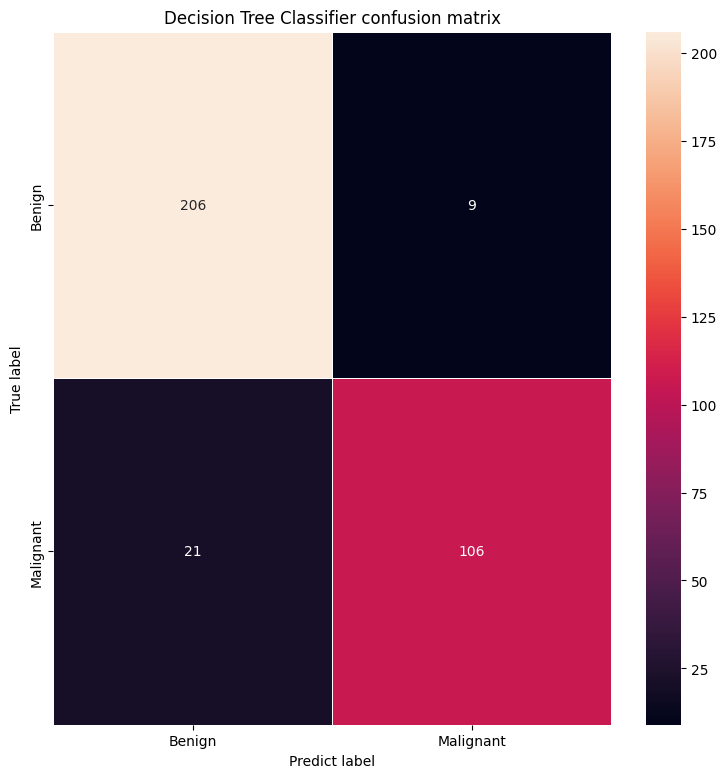
\includegraphics[width=\linewidth]{figures/dataset1/4060.png}
		\caption{Confusion Matrix với Train=40\% và Test=60\%}
		\label{fig:confusion_4060}
	\end{minipage}
\end{figure}

\[
\begin{bmatrix}
	\text{TP}_{B} = 206 & \text{FP}_{B} = 21 \\
	\text{FN}_{B} = 9   & \text{TP}_{M} = 106
\end{bmatrix}
\]

\begin{itemize}
	\item \textbf{True Positives (TP):}
	\begin{itemize}
		\item \textbf{Lớp B:} 206 mẫu B được dự đoán đúng là B.
		\item \textbf{Lớp M:} 106 mẫu M được dự đoán đúng là M.
	\end{itemize}
	
	\item \textbf{False Positives (FP):}
	\begin{itemize}
		\item \textbf{Lớp B:} 21 mẫu M bị dự đoán nhầm thành B.
		\item \textbf{Lớp M:} 9 mẫu B bị dự đoán nhầm thành M.
	\end{itemize}
	
	\item \textbf{False Negatives (FN):}
	\begin{itemize}
		\item \textbf{Lớp B:} 9 mẫu B bị nhầm thành M.
		\item \textbf{Lớp M:} 21 mẫu M bị nhầm thành B.
	\end{itemize}
\end{itemize}

\textbf{Nhận xét:}
\begin{itemize}
	\item \textbf{Hiệu suất mô hình:}
	\begin{itemize}
		\item Mô hình hoạt động \textbf{tốt trên nhãn B} với số lượng \textbf{True Positives (TP)} rất cao: 206/215.
		\item Chỉ có 9 \textbf{False Negatives (FN)} cho nhãn B $\rightarrow$ Recall của nhãn B rất cao (0.96), cho thấy mô hình ít bỏ sót các trường hợp thuộc nhãn này.
		\item Đối với nhãn M, mô hình có 106 \textbf{True Positives (TP)} nhưng có 21 \textbf{False Negatives (FN)} $\rightarrow$ Recall của nhãn M thấp hơn (0.83).
	\end{itemize}
	
	\item \textbf{Mất cân bằng dữ liệu:}
	\begin{itemize}
		\item Số lượng mẫu của nhãn B (\textbf{215}) lớn hơn nhãn M (\textbf{127}), tạo ra sự \textbf{mất cân bằng} trong dữ liệu.
		\item Điều này khiến mô hình có xu hướng ưu tiên dự đoán nhãn B hơn nhãn M, dẫn đến Recall thấp cho nhãn M.
	\end{itemize}
	
	\item \textbf{Tổng kết hiệu suất mô hình:}
	\begin{itemize}
		\item Mô hình đạt \textbf{Accuracy} = 0.91 $\rightarrow$ hiệu suất tổng thể rất tốt.
		\item Tuy nhiên, hiệu suất giữa hai nhãn \textbf{không cân bằng}:
		\begin{itemize}
			\item \textbf{Nhãn B:} Hoạt động xuất sắc với Recall và Precision cao.
			\item \textbf{Nhãn M:} Còn hạn chế với Recall thấp do số lượng \textbf{False Negatives (21)} lớn.
		\end{itemize}
	\end{itemize}
\end{itemize}


\subsubsection{Classification Report và Confusion Matrix (Train=60\%,Test=40\%)}

\textbf{Phân tích Classification Report}

\begin{table}[h!]
	\centering
	\begin{tabular}{|l|c|c|c|c|}
		\hline
		\textbf{} & \textbf{Precision} & \textbf{Recall} & \textbf{F1-Score} & \textbf{Support} \\ \hline
		\textbf{B} & 0.94 & 0.96 & 0.95 & 143 \\ \hline
		\textbf{M} & 0.93 & 0.91 & 0.92 & 85 \\ \hline
		\textbf{Accuracy} & \multicolumn{2}{c|}{} & 0.94 & 228 \\ \hline
		\textbf{Macro Avg} & 0.94 & 0.93 & 0.93 & 228 \\ \hline
		\textbf{Weighted Avg} & 0.94 & 0.94 & 0.94 & 228 \\ \hline
	\end{tabular}
	\caption{Classification Report với Train=60\% và Test=40\%.}
\end{table}

\begin{itemize}
	\item \textbf{Precision (Độ chính xác)}:  
	Precision đo lường tỷ lệ các dự đoán dương tính đúng trên tổng số dự đoán dương tính. Điều này phản ánh mức độ chính xác khi mô hình khẳng định một mẫu thuộc về một nhãn cụ thể.
	\begin{itemize}
		\item \textbf{B (0.94):} Precision cao cho thấy mô hình rất ít dự đoán nhầm các mẫu khác thành nhãn B.
		\item \textbf{M (0.93):} Precision của nhãn M đạt 93\%, chỉ thấp hơn một chút so với nhãn B. Điều này chứng tỏ mô hình có khả năng xác định chính xác nhãn M, dù số lượng mẫu của nhãn này ít hơn.
		\item \textbf{Trung bình (Macro Avg và Weighted Avg)}: \textbf{0.94}, phản ánh kết quả ổn định và cân bằng giữa các nhãn \textbf{B} và \textbf{M}.
	\end{itemize}
	
	\item \textbf{Recall (Độ nhạy)}:  
	Recall đo lường khả năng mô hình phát hiện đầy đủ các trường hợp dương tính thực tế. Chỉ số này đặc biệt quan trọng với các bài toán mà bỏ sót nhãn dương tính có thể gây ra rủi ro lớn.
	\begin{itemize}
		\item \textbf{B (0.96):} Với Recall đạt 96\%, mô hình phát hiện gần như tất cả các mẫu thực tế thuộc nhãn B. Điều này cho thấy mô hình rất nhạy trong việc nhận diện nhãn B và ít bỏ sót.
		\item \textbf{M (0.91):} Recall của nhãn M đạt 91\%, thấp hơn nhãn B. Điều này cho thấy mô hình còn bỏ sót khoảng 9\% các trường hợp thực tế thuộc nhãn M, có thể do nhãn này có ít dữ liệu hơn.
		\item \textbf{Trung bình (Macro Avg)}: \textbf{0.93} và \textbf{Weighted Avg}: \textbf{0.94} $\rightarrow$ mô hình hoạt động ổn định trên cả hai nhãn.
	\end{itemize}
	
	\item \textbf{F1-Score}:  
	F1-Score là trung bình điều hòa giữa Precision và Recall, giúp cân bằng giữa độ chính xác và độ nhạy.
	\begin{itemize}
		\item \textbf{B (0.95):} F1-Score của nhãn B đạt 0.95, phản ánh khả năng cân bằng rất tốt giữa Precision và Recall. Mô hình hoạt động hiệu quả và ít mắc sai sót với nhãn này.
		\item \textbf{M (0.92):} F1-Score của nhãn M đạt 0.92, thấp hơn một chút so với nhãn B do Recall thấp hơn. Mặc dù vậy, mô hình vẫn duy trì hiệu suất tốt cho nhãn này.
		\item \textbf{Trung bình (Macro Avg và Weighted Avg)}: \textbf{0.93 -- 0.94} cho thấy hiệu suất tổng thể tốt và mô hình không bị thiên lệch về một nhãn nào.
	\end{itemize}
	
	\item \textbf{Accuracy (Độ chính xác tổng thể)}:  
	Accuracy đạt \textbf{0.94}, nghĩa là mô hình dự đoán chính xác 94\% tổng số 228 mẫu. Đây là kết quả rất tốt và phản ánh độ tin cậy cao của mô hình trên cả hai nhãn.
\end{itemize}


\textbf{Phân tích Confusion Matrix}


\begin{figure}[h!]
	\centering
	\begin{minipage}[b]{0.43\linewidth}
		\centering
		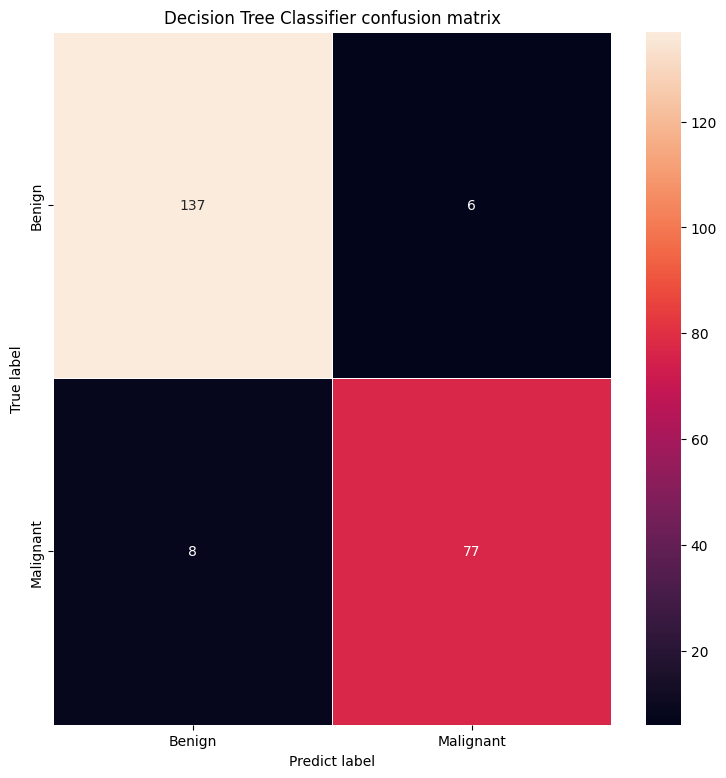
\includegraphics[width=\linewidth]{figures/dataset1/6040.png}
		\caption{Confusion Matrix với Train=60\% và Test=40\%}
		\label{fig:confusion_6040}
	\end{minipage}
\end{figure}

\[
\begin{bmatrix}
	\text{TP}_{B} = 137 & \text{FP}_{B} = 8 \\
	\text{FN}_{B} = 6   & \text{TP}_{M} = 77
\end{bmatrix}
\]

\begin{itemize}
	\item \textbf{True Positives (TP):}
	\begin{itemize}
		\item \textbf{Lớp B:} 137 mẫu B được dự đoán đúng là B.
		\item \textbf{Lớp M:} 77 mẫu M được dự đoán đúng là M.
	\end{itemize}
	
	\item \textbf{False Positives (FP):}
	\begin{itemize}
		\item \textbf{Lớp B:} 8 mẫu M bị dự đoán nhầm thành B.
		\item \textbf{Lớp M:} 6 mẫu B bị dự đoán nhầm thành M.
	\end{itemize}
	
	\item \textbf{False Negatives (FN):}
	\begin{itemize}
		\item \textbf{Lớp B:} 6 mẫu B bị nhầm thành M.
		\item \textbf{Lớp M:} 8 mẫu M bị nhầm thành B.
	\end{itemize}
\end{itemize}

\textbf{Nhận xét:}
\begin{itemize}
	\item \textbf{Hiệu suất mô hình:}
	\begin{itemize}
		\item Mô hình hoạt động \textbf{tốt trên nhãn B} với số lượng \textbf{True Positives (TP)} rất cao: 137/143.
		\item Chỉ có 6 \textbf{False Negatives (FN)} cho nhãn B $\rightarrow$ Recall của nhãn B rất cao (0.96).
		\item Đối với nhãn M, mô hình có 77 \textbf{True Positives (TP)} nhưng có 8 \textbf{False Negatives (FN)} $\rightarrow$ Recall của nhãn M thấp hơn một chút (0.91).
	\end{itemize}
	
	\item \textbf{Sự cân bằng giữa Precision và Recall:}
	\begin{itemize}
		\item Precision và Recall của nhãn B đều cao, chứng tỏ mô hình nhận diện tốt nhãn này.
		\item Precision và Recall của nhãn M vẫn khá tốt nhưng còn một số sai sót (FN=8 và FP=8), có thể cải thiện thêm.
	\end{itemize}
	
	\item \textbf{Tổng kết hiệu suất mô hình:}
	\begin{itemize}
		\item Mô hình đạt kết quả tốt với độ chính xác cao, đặc biệt trên nhãn B.
		\item Nhãn M hoạt động ổn định nhưng cần giảm tỷ lệ nhầm lẫn để tăng Recall và Precision.
	\end{itemize}
\end{itemize}



\newpage

\subsubsection{Classification Report và Confusion Matrix (Train=80\%,Test=20\%)}

\textbf{Phân tích Classification Report}

\begin{table}[h!]
	\centering
	\begin{tabular}{|l|c|c|c|c|}
		\hline
		\textbf{} & \textbf{Precision} & \textbf{Recall} & \textbf{F1-Score} & \textbf{Support} \\ \hline
		\textbf{B} & 0.95 & 0.99 & 0.97 & 72 \\ \hline
		\textbf{M} & 0.97 & 0.90 & 0.94 & 42 \\ \hline
		\textbf{Accuracy} & \multicolumn{2}{c|}{} & 0.96 & 114 \\ \hline
		\textbf{Macro Avg} & 0.96 & 0.95 & 0.95 & 114 \\ \hline
		\textbf{Weighted Avg} & 0.96 & 0.96 & 0.96 & 114 \\ \hline
	\end{tabular}
	\caption{Classification Report với Train=80\% và Test=20\%.}
\end{table}

\begin{itemize}
	\item \textbf{Precision (Độ chính xác)}:  
	Precision đo lường tỷ lệ dự đoán dương tính đúng trên tổng số dự đoán dương tính.
	\begin{itemize}
		\item \textbf{B (0.95):} Precision của nhãn B đạt 95\%, cho thấy mô hình rất ít nhầm lẫn khi dự đoán nhãn B.  
		\item \textbf{M (0.97):} Precision của nhãn M cao hơn nhãn B (97\%), chứng tỏ mô hình dự đoán rất chính xác cho nhãn M.
		\item \textbf{Trung bình (Macro Avg và Weighted Avg)}: \textbf{0.96} cho thấy kết quả chính xác và ổn định giữa các nhãn.
	\end{itemize}
	
	\item \textbf{Recall (Độ nhạy)}:  
	Recall đo lường khả năng mô hình phát hiện đầy đủ các trường hợp dương tính thực tế.
	\begin{itemize}
		\item \textbf{B (0.99):} Recall rất cao (99\%) cho thấy mô hình phát hiện gần như toàn bộ các mẫu thực tế thuộc nhãn B.  
		\item \textbf{M (0.90):} Recall của nhãn M chỉ đạt 90\%, thấp hơn nhãn B. Điều này cho thấy mô hình bỏ sót khoảng 10\% các trường hợp thực tế thuộc nhãn M.
		\item \textbf{Trung bình (Macro Avg):} \textbf{0.95} và \textbf{Weighted Avg:} \textbf{0.96}, thể hiện mô hình có khả năng phát hiện tốt trên cả hai nhãn.
	\end{itemize}
	
	\item \textbf{F1-Score}:  
	F1-Score là trung bình điều hòa giữa Precision và Recall, giúp cân bằng giữa độ chính xác và độ nhạy.
	\begin{itemize}
		\item \textbf{B (0.97):} F1-Score của nhãn B đạt 0.97, phản ánh hiệu suất rất tốt nhờ Recall cực cao và Precision ổn định.  
		\item \textbf{M (0.94):} F1-Score của nhãn M thấp hơn một chút (\textbf{0.94}) do Recall kém hơn so với Precision.  
		\item \textbf{Trung bình (Macro Avg):} \textbf{0.95} và \textbf{Weighted Avg:} \textbf{0.96} cho thấy mô hình đạt hiệu suất tổng thể cao.
	\end{itemize}
	
	\item \textbf{Accuracy (Độ chính xác tổng thể)}:  
	Accuracy đạt \textbf{0.96}, nghĩa là mô hình dự đoán chính xác 96\% trên tổng số \textbf{114} mẫu. Đây là kết quả rất tốt, cho thấy mô hình hoạt động ổn định trên cả hai nhãn.
\end{itemize}
\newpage
\textbf{Phân tích Confusion Matrix}
\begin{figure}[h!]
	\centering
	\begin{minipage}[b]{0.6\linewidth}
		\centering
		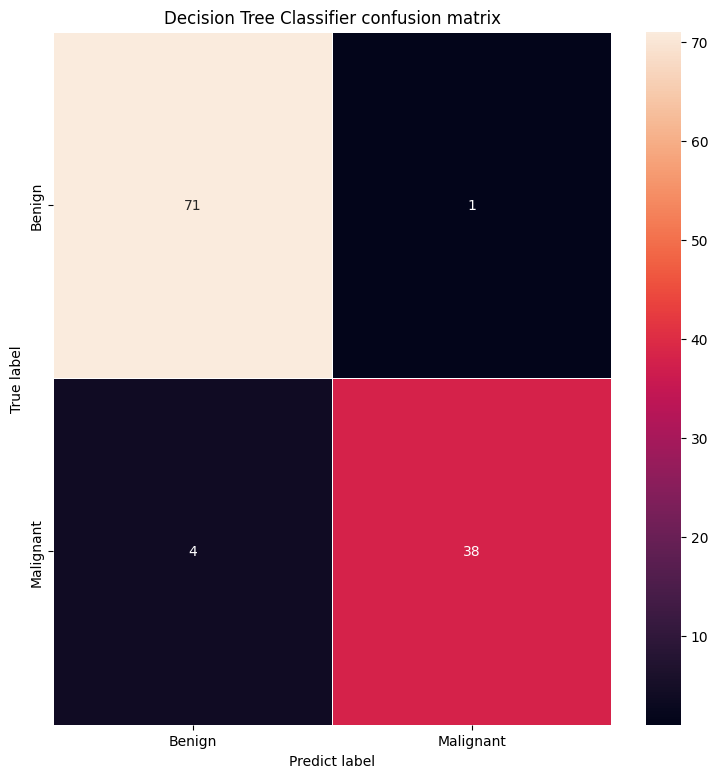
\includegraphics[width=\linewidth]{figures/dataset1/8020.png}
		\caption{Confusion Matrix với Train=80\% và Test=20\%}
		\label{fig:confusion_8020}
	\end{minipage}
\end{figure}

\[
\begin{bmatrix}
	\text{TP}_{B} = 71 & \text{FP}_{B} = 4 \\
	\text{FN}_{B} = 1   & \text{TP}_{M} = 38
\end{bmatrix}
\]

\begin{itemize}
	\item \textbf{True Positives (TP):}
	\begin{itemize}
		\item \textbf{Lớp B:} 71 mẫu B được dự đoán đúng là B.
		\item \textbf{Lớp M:} 38 mẫu M được dự đoán đúng là M.
	\end{itemize}
	
	\item \textbf{False Positives (FP):}
	\begin{itemize}
		\item \textbf{Lớp B:} 4 mẫu M bị dự đoán nhầm thành B.
		\item \textbf{Lớp M:} 1 mẫu B bị dự đoán nhầm thành M.
	\end{itemize}
	
	\item \textbf{False Negatives (FN):}
	\begin{itemize}
		\item \textbf{Lớp B:} 1 mẫu B bị nhầm thành M.
		\item \textbf{Lớp M:} 4 mẫu M bị nhầm thành B.
	\end{itemize}
\end{itemize}

\textbf{Nhận xét:}
\begin{itemize}
	\item \textbf{Hiệu suất mô hình:}
	\begin{itemize}
		\item \textbf{Nhãn B:} Mô hình hoạt động rất tốt với \textbf{True Positives (TP)} cao (\textbf{71/72}), chỉ có 1 \textbf{False Negative (FN)} $\rightarrow$ Recall đạt \textbf{0.99}.
		\item \textbf{Nhãn M:} Mô hình có \textbf{38 True Positives (TP)} nhưng vẫn còn 4 \textbf{False Negatives (FN)}, khiến Recall đạt \textbf{0.90}.
	\end{itemize}
	
	\item \textbf{Sự cân bằng Precision và Recall:}
	\begin{itemize}
		\item Precision của nhãn B rất cao do số lượng False Positives (FP) nhỏ.
		\item Recall của nhãn M (\textbf{0.90}) tuy tốt nhưng thấp hơn nhãn B (\textbf{0.99}) do số lượng \textbf{False Negatives (FN)} còn tồn tại.
	\end{itemize}
	
	\item \textbf{Tổng kết hiệu suất mô hình:}
	\begin{itemize}
		\item Độ chính xác tổng thể của mô hình rất cao với số lượng nhầm lẫn rất nhỏ.
		\item \textbf{Accuracy cao và hiệu suất tốt trên cả hai nhãn}, đặc biệt là nhãn B.
		\item Mô hình có thể cải thiện Recall của nhãn M bằng cách giảm \textbf{False Negatives}.
	\end{itemize}
\end{itemize}



\subsubsection{Classification Report và Confusion Matrix (Train=90\%,Test=10\%)}

\textbf{Phân tích Classification Report}
\begin{table}[h!]
	\centering
	\begin{tabular}{|l|c|c|c|c|}
		\hline
		\textbf{} & \textbf{Precision} & \textbf{Recall} & \textbf{F1-Score} & \textbf{Support} \\ \hline
		\textbf{B} & 0.95 & 0.97 & 0.96 & 36 \\ \hline
		\textbf{M} & 0.95 & 0.90 & 0.93 & 21 \\ \hline
		\textbf{Accuracy} & \multicolumn{2}{c|}{} & 0.95 & 57 \\ \hline
		\textbf{Macro Avg} & 0.95 & 0.94 & 0.94 & 57 \\ \hline
		\textbf{Weighted Avg} & 0.95 & 0.95 & 0.95 & 57 \\ \hline
	\end{tabular}
	\caption{Classification Report với Train=90\% và Test=10\%.}
\end{table}

\begin{itemize}
	\item \textbf{Precision (Độ chính xác)}:  
	Precision đo tỷ lệ các dự đoán dương tính đúng trên tổng số dự đoán dương tính.
	\begin{itemize}
		\item \textbf{B (0.95):} Precision của nhãn B đạt \textbf{95\%}, cho thấy mô hình dự đoán chính xác hầu hết các trường hợp thuộc nhãn này.
		\item \textbf{M (0.95):} Precision của nhãn M cũng đạt \textbf{95\%}, phản ánh độ chính xác tương đương với nhãn B.
		\item \textbf{Trung bình (Macro Avg và Weighted Avg):} Cả hai giá trị đều là \textbf{0.95}, chứng tỏ mô hình dự đoán ổn định và cân bằng giữa các nhãn.
	\end{itemize}
	
	\item \textbf{Recall (Độ nhạy)}:  
	Recall phản ánh khả năng phát hiện đầy đủ các trường hợp dương tính thực tế.
	\begin{itemize}
		\item \textbf{B (0.97):} Recall của nhãn B đạt \textbf{97\%}, nghĩa là mô hình gần như phát hiện toàn bộ các mẫu thực tế thuộc nhãn B.
		\item \textbf{M (0.90):} Recall của nhãn M thấp hơn (\textbf{90\%}), cho thấy khoảng \textbf{10\%} các trường hợp nhãn M bị bỏ sót.  
		\item \textbf{Trung bình (Macro Avg):} \textbf{0.94} cho thấy mức độ phát hiện tổng thể trên cả hai nhãn vẫn tốt nhưng bị ảnh hưởng bởi Recall của nhãn M.
	\end{itemize}
	
	\item \textbf{F1-Score}:  
	F1-Score là trung bình điều hòa giữa Precision và Recall, giúp cân bằng độ chính xác và độ nhạy.
	\begin{itemize}
		\item \textbf{B (0.96):} F1-Score của nhãn B đạt \textbf{0.96}, phản ánh hiệu suất rất cao với độ chính xác và độ nhạy tốt.
		\item \textbf{M (0.93):} F1-Score của nhãn M đạt \textbf{0.93}, thấp hơn nhãn B do Recall còn hạn chế.
		\item \textbf{Trung bình (Macro Avg):} \textbf{0.94} và \textbf{Weighted Avg:} \textbf{0.95}, chứng tỏ mô hình hoạt động hiệu quả trên toàn bộ tập dữ liệu.
	\end{itemize}
	
	\item \textbf{Accuracy (Độ chính xác tổng thể)}:  
	Accuracy đạt \textbf{0.95}, nghĩa là mô hình dự đoán chính xác 95\% trên tổng số \textbf{57} mẫu. Đây là kết quả rất tốt, phản ánh khả năng tổng quát hóa tốt của mô hình trên tập dữ liệu test.
\end{itemize}

\textbf{Phân tích Confusion Matrix}
\begin{figure}[h!]
	\centering
	\begin{minipage}[b]{0.6\linewidth}
		\centering
		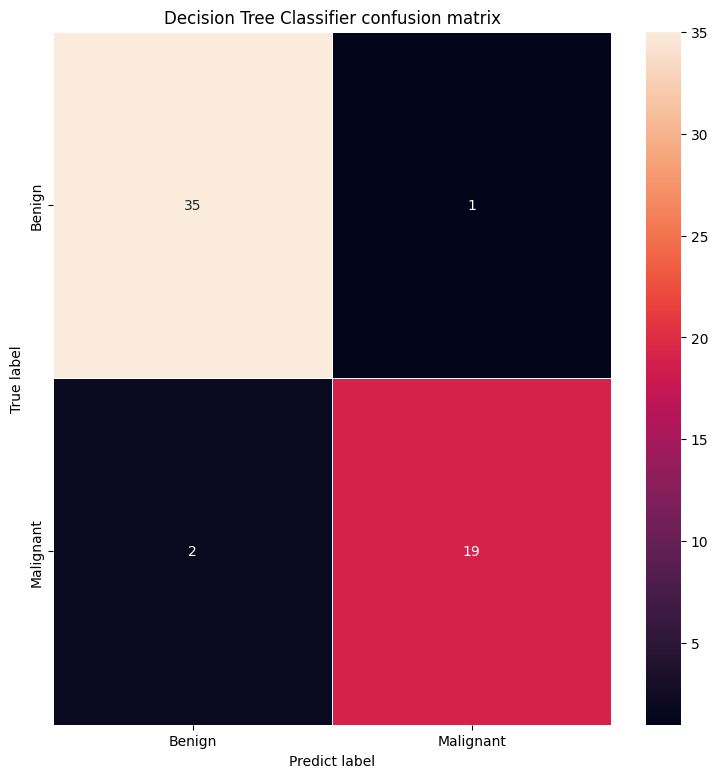
\includegraphics[width=\linewidth]{figures/dataset1/9010.png}
		\caption{Confusion Matrix với Train=90\% và Test=10\%}
		\label{fig:confusion_9010}
	\end{minipage}
\end{figure}

\[
\begin{bmatrix}
	\text{TP}_{B} = 35 & \text{FP}_{B} = 2 \\
	\text{FN}_{B} = 1   & \text{TP}_{M} = 19
\end{bmatrix}
\]

\begin{itemize}
	\item \textbf{True Positives (TP):}
	\begin{itemize}
		\item \textbf{Lớp B:} 35 mẫu B được dự đoán đúng là B.
		\item \textbf{Lớp M:} 19 mẫu M được dự đoán đúng là M.
	\end{itemize}
	
	\item \textbf{False Positives (FP):}
	\begin{itemize}
		\item \textbf{Lớp B:} 2 mẫu M bị dự đoán nhầm thành B.
		\item \textbf{Lớp M:} 1 mẫu B bị dự đoán nhầm thành M.
	\end{itemize}
	
	\item \textbf{False Negatives (FN):}
	\begin{itemize}
		\item \textbf{Lớp B:} 1 mẫu B bị nhầm thành M.
		\item \textbf{Lớp M:} 2 mẫu M bị nhầm thành B.
	\end{itemize}
\end{itemize}

\textbf{Nhận xét:}
\begin{itemize}
	\item \textbf{Hiệu suất mô hình:}
	\begin{itemize}
		\item \textbf{Nhãn B:} Mô hình hoạt động rất tốt với \textbf{True Positives (TP)} đạt \textbf{35/36}, chỉ có 1 \textbf{False Negative (FN)}. Điều này giúp Recall của nhãn B đạt \textbf{0.97}.
		\item \textbf{Nhãn M:} Mô hình có \textbf{19 True Positives (TP)} nhưng còn 2 \textbf{False Negatives (FN)}, làm Recall của nhãn M giảm xuống \textbf{0.90}.
	\end{itemize}
	
	\item \textbf{Sự cân bằng Precision và Recall:}
	\begin{itemize}
		\item Precision của nhãn B rất cao do số lượng False Positives (FP) nhỏ (\textbf{2}).
		\item Precision và Recall của nhãn M còn cải thiện được bằng cách giảm False Negatives (\textbf{2}) và False Positives (\textbf{1}).
	\end{itemize}
	
	\item \textbf{Tổng kết hiệu suất mô hình:}
	\begin{itemize}
		\item Độ chính xác tổng thể của mô hình rất cao với mức nhầm lẫn rất nhỏ.
		\item Nhãn B có độ chính xác và độ nhạy cao vượt trội.
		\item Nhãn M cũng có hiệu suất tốt nhưng cần tối ưu để giảm thiểu số lượng False Negatives.
	\end{itemize}
\end{itemize}



\subsection{Phân tích độ sâu và độ chính xác}

\begin{table}[h!]
	\centering

	\label{tab:max_depth_accuracy}
	\begin{tabular}{|l|c|c|c|c|c|c|c|c|}
		\hline
		\textbf{max\_depth} & \textbf{None} & \textbf{2} & \textbf{3} & \textbf{4} & \textbf{5} & \textbf{6} & \textbf{7} \\ \hline
		\textbf{Accuracy}   & 0.9561 & 0.8860 & 0.9386 & 0.9298 & 0.9561 & 0.9298 & 0.9561 \\ \hline
	\end{tabular}
	\caption{Độ chính xác với từng giá trị max\_depth.}
\end{table}

\newpage
\begin{figure}[h!]
	\centering
	\begin{tikzpicture}
		\begin{axis}[
			title={Biểu đồ độ chính xác theo max\_depth},
			xlabel={max\_depth},
			ylabel={Accuracy},
			xtick={0,2,3,4,5,6,7},
			ymin=0.88, ymax=0.97,
			grid=both,
			width=0.8\linewidth,
			height=0.5\linewidth,
			legend style={at={(0.97,0.03)}, anchor=south east},
			ymajorgrids=true
			]
			\addplot[color=blue,mark=square*,line width=1pt] coordinates {
				(0, 0.9561) % None
				(2, 0.8860)
				(3, 0.9386)
				(4, 0.9298)
				(5, 0.9561)
				(6, 0.9298)
				(7, 0.9561)
			};
			\legend{Accuracy}
		\end{axis}
	\end{tikzpicture}
	\caption{Biểu đồ độ chính xác của mô hình cây quyết định với từng giá trị max\_depth.}
	\label{fig:max_depth_accuracy}
\end{figure}


\textbf{Nhận xét:}
\begin{itemize}
	\item \textbf{max\_depth = None:} Độ chính xác đạt \textbf{0.9561}, rất cao. Không giới hạn độ sâu giúp mô hình phân tách hoàn hảo nhưng có thể dẫn đến quá khớp (overfitting).
	
	\item \textbf{max\_depth = 2:} Độ chính xác giảm xuống \textbf{0.8860}. Điều này cho thấy mô hình quá đơn giản, không đủ độ sâu để phân tách dữ liệu chính xác.
	
	\item \textbf{max\_depth = 3:} Độ chính xác tăng lên \textbf{0.9386}. Mô hình cải thiện so với `max\_depth = 2` nhưng vẫn chưa đạt hiệu suất tối đa.
	
	\item \textbf{max\_depth = 4:} Độ chính xác giảm nhẹ còn \textbf{0.9298}, sự cân bằng giữa underfitting và overfitting chưa được tối ưu.
	
	\item \textbf{max\_depth = 5:} Độ chính xác quay lại mức cao nhất là \textbf{0.9561}, cho thấy đây có thể là độ sâu tối ưu cho mô hình này.
	
	\item \textbf{max\_depth = 6:} Độ chính xác giảm nhẹ xuống \textbf{0.9298}, cho thấy mô hình có thể đã bắt đầu xuất hiện dấu hiệu của quá khớp.
	
	\item \textbf{max\_depth = 7:} Độ chính xác đạt lại \textbf{0.9561}, giống với `max\_depth = 5`. Mức này đảm bảo mô hình hoạt động tốt nhưng cần kiểm tra thêm để tránh quá khớp(overfitting).
\end{itemize}

